\documentclass{standalone}
\usepackage{amsmath, mathrsfs}

\usepackage{tikz}
\usetikzlibrary{shapes, calc}


\tikzset{
	myblocktext/.style={rectangle, top color=red!20!white, bottom color=red!70!black!90, rounded corners=2mm, minimum height=0.5cm,
				inner sep=0.1cm,  text centered, align=center,
				font=\small, text=white
				},
	myblockeqs/.style={rectangle, top color=gray!10, bottom color=gray!50, rounded corners=2mm, 
				inner sep=0.1cm,  text centered, align=center,
				text=black
				},	
	myblockdecision/.style={diamond, inner sep=0mm, text badly centered, minimum height=1cm, minimum width=3.00cm,
				rounded corners=3mm, draw=none, top color=yellow!50, bottom color=yellow!50!black
				},	
	myarrow/.style={->, black, >=latex, shorten >=2pt, shorten <=2pt, line width=1pt, opacity = 0.5
				},
	mylabeliter/.style={inner sep=0mm, text badly centered, minimum height=0.25cm, minimum width=1.00cm,
				rounded corners=3mm, draw=none, top color=orange!7, bottom color=orange!30
				},
	blockend/.style={inner sep=0mm, text badly centered, minimum height=0.4cm, minimum width=1.00cm,
				rounded corners=1mm, draw=none, top color=green!20, bottom color=green!50!black
				}
	}
				
\newcommand\rvec{\mathbf{r}}

\begin{document}
	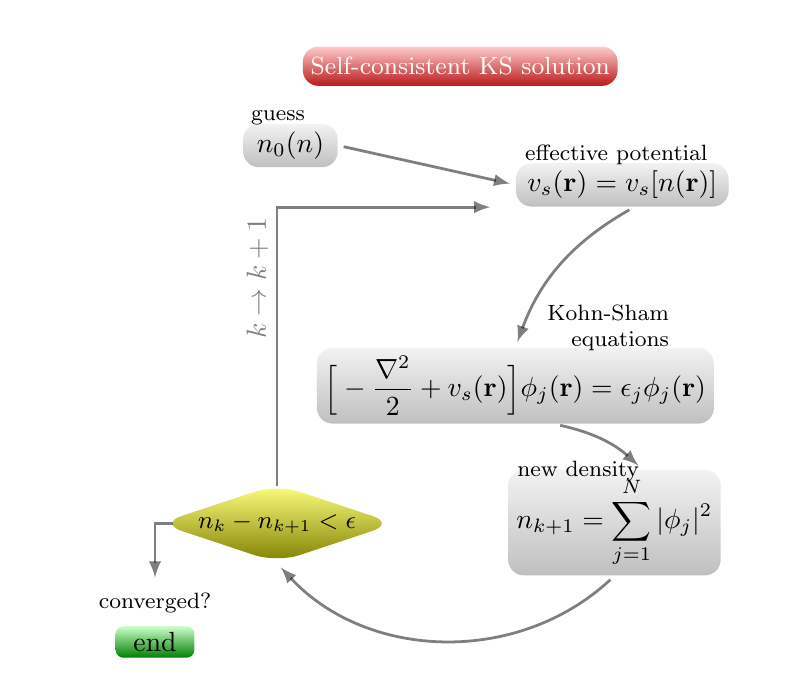
\begin{tikzpicture}

				\node[] (origem) at (0,0) {}; 
				
				\node[] (fantasma) at ($(origem) + (1.0, 1.0)$) {\vphantom{h}};
				
				\node[myblocktext] (KSDFT) at ($(fantasma) + (2.5, -0.25)$) {Self-consistent KS solution};
				
				\node[myblockeqs] (n0) at 
				($(KSDFT.south west) + (-0.15,-0.75)$) [text width=1cm, align=center] {$n_0(n)$};
				\node[anchor=south] (n0t) at ($(n0.north) + (0,-0.15)$) [text width=1cm, font=\footnotesize] {guess};
				
				\node[anchor=west, myblockeqs] (Veffn) at 
				($(n0.east) + (2.25, -0.5)$) [text width=2.5cm, align=center]
				{$\displaystyle v_{s} (\mathbf{r}) = v_s[n (\rvec)]$};
				
				
				\node[anchor=south west] (Veffnt) at ($(Veffn.north west) + (0, -0.15)$) [text width=3cm, font=\footnotesize, align=left]
				{effective potential};
				
				
				\node[myblockeqs] (KSeq) at ($(n0.east) + (2.25, -3.05)$) 
				{$\displaystyle \Big[ -\frac{\nabla^2}{2} + v_{s}(\mathbf{r}) \Big] \phi_j(\mathbf{r}) = \epsilon_j \phi_j(\mathbf{r})  
$};
				\node[anchor=south] (KSeqt) at ($(KSeq.north) + (0.95, -0.175)$) 
				[text width=2cm, font=\footnotesize, align=right]
				{Kohn-Sham equations};


				\node[anchor=west, myblockeqs] (nk) at 
				($(KSeq.south) + (-0.1, -1.25)$) [text width=2.5cm, align=center]
				{$\displaystyle n_{k+1}=  \sum_{j=1}^{N} |\phi_j|^2  $ };
				
				
				\node[anchor=south west] (nkt) at ($(nk.north west) + (-0.0, -0.275)$) [text width=3cm, font=\footnotesize, align=left]
				{new density};				 
				
				\node [myblockdecision] 
				(converge) at ($(KSeq.west) + (-0.5,-1.75)$) {};
				
				\node [] 
				(converget) at ($(converge.center) + (0,0)$)[font=\small] {$n_k - n_{k+1} < \epsilon$};
				

		
				\node[anchor=north] (convergett) at ($(converge.south) + (-1.55, -0.25)$) 
				[text width=3cm, font=\footnotesize, align=center]
				{converged?};	
				
				\node[blockend] (convergeyes) at ($(convergett.south) + (0.,-0.25)$) {end};
				
				\draw[myarrow]  ($(converge.west)+(0.25,0)$) -| node [near start, left] {} (convergett.north) ;
				
				\draw[myarrow] ($(n0.east) + (0, 0)$) to node[bend left=45] {}($(Veffn.west)+(0,0)$);     	

				\draw[myarrow,  bend left=-20]
				($(Veffn.south) + (0.15, 0)$) to node[] {}($(KSeq.north)+(0,0)$);     	
				
				\draw[myarrow, bend left=15] 
				($(KSeq.south) + (0.5, 0)$) to node[] {}($(nk.north east)+(-1,0)$);  
				
				\draw[myarrow, bend left=45]  
				(nk.south) to node[bend left=45] {} (converge.south);           		
		
				\draw[myarrow]  ($(converge.north)+(0.0, -0.1)$)  |-
				 node[left, xshift=-0.25cm, rotate=90] {$k \rightarrow k+1$} 
				 ($(Veffn.south west) +(-0.25,0)$);           		
		
		
	\end{tikzpicture}
\end{document}
